      \subsection{Nástroje pro replikaci v PostgreSQL}

      PostgreSQL nabízí hned několik nástrojů pro řešení replikace. Je možno použít zabudovanou streaming replikaci, která je dostupná od verze PostgreSQL 9.0 nebo některou z extenzí, například Slony-I, pgpool, Londiste, Bucardo nebo Postgres-XC, pro jejichž srovnání \vizTabulka{tSrovnaniReplikace}. Tato kapitola se dále bude zabývat a porovnávat nativní streaming replikace s extenzí Slony-I a pgpool.

        \begin{table}[H]
          \caption{Srovnání různých typů dostupných replikačních řešení}
          \label{tSrovnaniReplikace}
          \begin{footnotesize}
            \begin{center}
              \rowcolors{1}{white}{lightgray}
              \begin{tabular}{|c|cccccc|}
                \hline
                {\bf \color{purpurova7}nástroje}	& {\bf \color{purpurova7}typ} & {\bf \color{purpurova7}technika} & {\bf \color{purpurova7}M/M} & {\bf \color{purpurova7}M/S} & {\bf \color{purpurova7}sync} & a{\bf \color{purpurova7}sync} \\
                \hline
                PostgreSQL 9.1* & fyzická & xlog & ne & ano & ano & ano \\
                     pgpool-II & logická & proxy & ano & ne & ano & ne \\
                       slony-I & logická & triggers & ne & ano & ne & ano \\
                      Londiste & logická & triggers & ne & ano & ne & ano \\
                       Bucardo & logická & triggers & ano & ano & ne & ano \\
                   Postgres-XC & cluster & - & ano & ne & ne & ano \\
                \hline
                \multicolumn{3}{l}{\scriptsize{*streaming replikace}} & \multicolumn{4}{r}{\scriptsize{zdroj: Tomáš Vondra, 2011}}\\
              \end{tabular}
            \end{center}
          \end{footnotesize}
        \end{table}

      \subsubsection{Slony-I}
      \label{kSlony}

      Jak píší \cite{Boszormenyi2013} je Slony-I jeden z nejrozšířenějších externích nástrojů pro replikaci pro PostgreSQL. Zároveň se také řadí mezi nejstarší, plně používán je v PostgreSQL již od verze 7.3. a je velmi dobře podporován i dalšími externími řešeními pro PostgreSQL, například programem PgAdmin3, který nabízí správu dat pomocí grafického rozhraní \citep{Boszormenyi2013}.

Jedná se o trigger-based replikaci, což znamená, že je ke každé exitující tabulce přidán trigger, který zajistí replikaci každé změny, která v databázi nastane. Z toho také vyplývá, že se jedná o logickou replikaci, kdy je možné replikovat pouze změny v datech, tzv. DML změny, tedy SQL příkazy INSERT a UPDATE, nikoli strukturu databáze, příkazy typu CREATE/DROP TABLE, ALTER TABLE. Každá změna struktury se tedy musí provést ručně, což se může jevit jako nevýhodné. Nese to ale i své klady, například možnost výběru pouze některých tabulek. Vytváří si totiž tzv. {\it replikační set}, do kterého se zapíší pouze ty tabulky, které je potřeba replikovat. 

Další výhodou, a to zvlášť v porování se streaming replikací, je možnost replikace dat mezi různými verzemi PostgreSQL bez ohledu na platformu a architekturu. Naopak spíše za nevýhodu je považováno, že si vytváři ke každé tabulce vlastní schéma, do kterého se ukládají replikovaná data, což způsobuje redundanci dat. 

Slony-I replikace je z principu asynchronní, zpoždění je v řádu jednotek či desítek vteřin. Umožňuje Hot Standby mode, kdy je možno použít repliku na dotazy, i kaskádovou replikaci. Slony-I má vlastní konfigurační nástroj a samotná replikace funguje díky vlastnímu replikačnímu démonu, který běží stále, registruje změny a kopíruje je na slave servery.

      \subsubsection{Streaming replikace}
      \label{kStreaming}

      Streaming replikace je nativní řešení do PostgreSQL implementované od verze 9.0. Jedná se o log-shipping replikaci, což znamená, že jsou na slave servery posílány transakční logy, v PostgreSQL nazývané WAL (Write Ahead Log). Do nich jsou změny nejdříve zaznamenávány přímým zápisem na disk a až poté potvzeny jako úspěšné. Tento způsob zajišťuje datům naprosté bezpečí, protože kdyby došlo k chybě a změny se nezapisovaly na disk, ale pouze do cache, mohlo by dojít k jejich ztrátě. Zároveň to zajišťuje kopii jak dat, tak i struktury databáze. Existuje pouze jeden transakční log pro jednu instalaci PostgreSQL, proto se replikují vždy všechny databáze a není možné výběru jen několika tabulek, tak jako u Slony-I \citep{Boszormenyi2013}. Protože replikace probíhá pomocí transakčního logu, je nutné použití stejné verze PostgreSQL, stejné platformy i architektury na všech uzlech replikačního clusteru. 

Streaming replikace umožňuje jak synchronní, tak asynchronní replikaci, dále Hot standby mode i kaskádovou replikaci.

      \subsubsection{pgpool}
      \label{kpgpool}

      Nástroj pgpool, který je stejně jako Slony-I extenzí pro PostgreSQL, je dalším z nástrojů, který je možno použít pro replikaci dat, umožňuje však i další pokročilé funkce jakými jsou sdílení spojení klienta s databází (angl. connection pooling), paralelní uložení dat (angl. parallel query) a rozložení zátěže mezi více servery (angl. load balancing) . 
pgpool umožňuje sdílení spojení klienta s databází, což v praxi znamená, že se vytvoří několik spojení se serverem, která i po skončení dotazu zůstanou otevřená a připravená pro další použití. Nemusí se tedy navazovat spojení při každém požadavku ze strany klienta, což velice zrychlí provoz a zajistí plynulost užívání databáze. Je vhodným nástrojem pro správu velkých tabulek díky distribuovanému způsobu ukládání dat \citep{pgpool2014}. 

Zároveň je nástrojem pro zjednodušení nastavení a provozu replikace a umožňuje rozložení zátěže mezi více serverů v replikačním clusteru, aby nedocházelo k přetíže jednotlivých uzlů a celkově se zvýšila rychlost a efektivita práce s databází. V případě rozložení zátěže se pgpool stává prostředníkem pro komunikaci mezi klientem a serverem. Aby nebylo potřeba dát každému uživateli přístup k jinému slave serveru, nebo přístupy do databáze manuálně rozkládat skrze složité programové řešení, nabízí se možnost použití pgpool, který se navenek jeví jako jakákoliv jiná databáze, do které se uživatelé připojí bez ohledu na jejich práva a požadavky. pgpool pak sám rozdělí dotazy mezi uzly v replikačním clusteru dle aktuální zátěže \citep{Boszormenyi2013}. Zároveň, pokud má uživatel přístup k zápisu i čtení, umí na základě jeho aktuálního SQL příkazu, rozhodnout, zda jej připojí k master nebo slave databázi, \odkazObrazek{opgpool}. Tento způsob velmi zjednoduší jak administraci databáze, tak nastavení pro běžného uživatele, který se připojí pouze do jedné databáze a víc se nezajímá, zda z databáze pouze čte, nebo do ní i zapisuje. 

Na základě vybraných funkcí je možno použít jeden ze čtyř základních módů, které pgpool poskytuje\footnote{kompletní přehled na \url{http://www.pgpool.net/docs/latest/pgpool-en.html\#config}}: základní, replikační, master/slave a paralelní. V návrh databázového řešení byl použit mód master/slave, který je dále popisován v kapitole \odkazKapitola{kpgpool}.

      \begin{figure}[H]
        \centering
        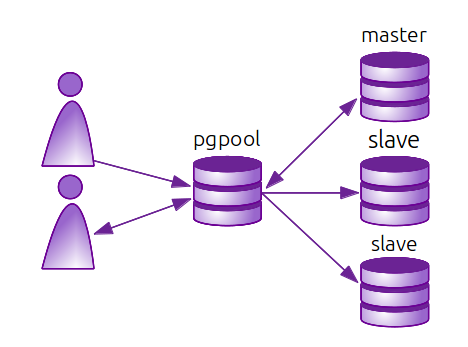
\includegraphics[scale=1]{../../../grafy/obr/schema_pgpool.png}
        \caption{Zjednodušené schéma pgpool v módu master/slave}
        \label{opgpool}
      \end{figure}

